\documentclass[12pt]{article}

\usepackage{cite}
\usepackage{amsmath,amssymb,amsfonts}
\usepackage{algorithmic}
\usepackage{graphicx}
\usepackage{textcomp}
\usepackage{xcolor}
\usepackage{float}

\begin{document}

\title{\textbf{Self-playing Snake Game based on Pathfinding Algorithms}}
\author{Yang Sui \and Jin Xu \and Runlin Hou}

\maketitle

\section{The Snake Game}
Before we implement the algorithms, we first need to build a snake game as a platform. Our design is to use graph theory to implement the snake game. 

We separate the snake game into three parts:
\begin{itemize}
    \item map
    \item snake
    \item food
\end{itemize}

The map is where the snake takes its movement, so we will build the map as the fundamental graph. Considering the structure of the map, it is like a  chessboard with blocks arranged in rows and columns that are perpendicular to each other. Each block of the map will be treated as a vertice, and the edges will be used to describe the connection of two vertices. 

For the body of the snake, since the blocks that the body was taken are unreachable for the snake. So we decide to mark those vertices as taken.

The food of the position will be saved. But the vertice itself will be the same as the other vertices since the food must be reachable for the snake to take.

As a whole, the snake game will be built on an undirected graph with the same weight for all edges. Because the snake would be able to reach every vertice, and each vertice will only take one movement to move to its adjacent vertice.

In the implementation of our snake on graph theory, all three parts can be built as follow:
\begin{itemize}
    \item map, an undirected and unweighted map
    \item snake, will be marked as unreachable vertice to its adjacencies
    \item food, normal vertice but the position will be saved
\end{itemize}

For the code implementation, we found that the map of the snake follows strict mathematical rules like every row has the same vertices, and also every column has the same vertices. Mathematically, each vertice's position can be calculated by adding or subtracting a certain value. Considering this situation, we save the whole map in a list and make a judgment of their connection according to their coordinates.

\section{BFS Approach}
Before I choose to use BFS as the algorithm, I actually think about some other ways to achieve my goals, like DFS or Dijkstra. For DFS, it will keep going on one path until it reaches the target. And renew this path if the other path is shorter. So with the map getting bigger, it will take much longer than the BFS. As for Dijkstra, when facing an undirected graph with the same weights for all edges, Dijkstra is exactly BFS. So I take BFS instead.

\begin{figure}[H]
    \centering 
    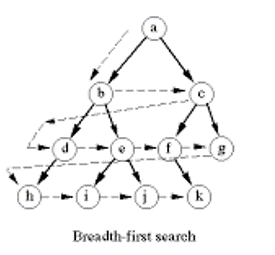
\includegraphics[scale = 0.8]{1.png}
    \caption{BFS algorithm}
    \label{fig:figure1}
\end{figure}

\subsection{Introduction}
We will start by talking about some common sense of the BFS algorithm. We all know that the BFS algorithm will traversal all of the vertices to find the target that we are looking for. If we are doing a BFS in a tree, and we search from the root node, the BFS algorithm can be seen as searching layer by layer from top to bottom. When we deal with a graph, we need to set an initial vertice for the algorithm and the process of the algorithm will spread like a water wave.

So generally speaking, the basic logic of the BFS algorithm is to set up an initial vertice and keep visiting the adjacencies until we find the target. 

\subsection{Implementation}
The implementation of the BFS is simple. And since we are dealing with an undirected graph with the same weight for edges. The process becomes easier. Considering the attribute of the BFS itself, every path found by BFS would be exactly the shortest path to the target because every vertice will be immediately added to the queue right after their parents been visited.

I use two functions to implement the kernel goal of the BFS algorithm. 
\begin{itemize}
    \item \verb|connected(vertice)|
    \item \verb|bfs(head, target)|
\end{itemize}

\verb|connect(ver)| will take a vertice as an input. And the output is a list of the adjacencies of this vertice. As we mentioned in the last section, the graph that our map mapped to is a list. Also, as we knew, the map of the Snake Game is like a chessboard, that each node has four edges and is vertical to each other. So the mathematical relationship of connected vertices can be described as following:

$a$, $b$ are coordinates of two vertices, when $a$, $b$ can fit the following equtoins, then they
are connected. $w$ is the length of the map.
\begin{eqnarray}
        a = b - 1 \\
        a = b + 1 \\
        a = b - w \\
        a = b + w 
\end{eqnarray}

Also during the judgment, we need to exclude the walls and the body of the snake, since they 
will be treated as unreachable vertices of the map. This can be easily achieved because we 
store the index of them as attributes in the \verb|solver| class.

\verb|bfs(head, target)| takes the head position of the snake and the target position as 
inputs. And it will return the shortest path from the snake's head to the target. 
To achieve the purpose of BFS, we first need to create a FIFO queue to record the incoming 
vertices. Each time we visited a new vertice, we will add its adjacencies into the queue for 
future visiting. This can be done easily combined with the \verb|connected(ver)|. 
Basically, the process will be going as visiting the vertices whose distance is 1 to head, 
and visited the vertices whose distance is 2 to head and so on. Once we reach the target, 
we will stop the loop.

\subsection{Strategy}

The kernel of the algorithm is to find the shortest path to the food. But it is not enough to
find the shortest path for the snake. Also, we need to tell the snake how it can try to be 
alive, so that snake can get more scores. 

I have the snake to follow three rules for the entire game. The first one is to find the food. 
As long as the snake can reach the food, it will go for it directly. But of course, with the 
game going on, the body of the snake might block the food from the head. This is when the snake
can not reach the food. And here comes the second rule that when the snake can not reach the 
food, it will chase the tail. And of course, there will also be a situation that the snake can
not found the food nor the tail. When we are facing this situation, I'll ask the sanke to move 
randomly and pray for the food can be reached several movements later.

Also, it is obvious that the game is a dynamic process. But the path we found is always based on a map in a certain moment. This means that we may not get the shortest path cause with the movement of snakes body, the connection of each vertice might be updated, then some new path will be created. So I will have the snake find a new path after every movement, though the first path can lead the snake to destination.

\section{Hamiltonian Circle Algorithm}

For above algorithms, they can't finish the game in the situation that the entire map is full of snake body, which means the snake can't eat every food. To solve this problem, I introduce a Hamiltonian Circle and use this into self-playing game to insure the snake can eat every food to the last. Furthermore, I'll put forward advanced Hamiltonian Circle Algorithm adding shortcuts in the naive Hamiltonian Circle Algorithm. There are two mainly contribution in Hamiltonian Circle Algorithm:
\begin{enumerate}
    \item Building the Hamilton Circle Algorithm to eat every food generated by random positions in the map. 
    \item Optimizing the Hamilton Circle Algorithm by adding shortcuts in early-stage.
\end{enumerate}
    
\subsection{Hamiltonian Circle}
In the mathematical field of graph theory, a Hamiltonian path (or traceable path) is a path in an undirected or directed graph that visits each vertex exactly once. A Hamiltonian cycle (or Hamiltonian circuit) is a Hamiltonian path that is a cycle. In \ref{fig:figure1label}, the red path is Hamiltonian Circle. 
    
\begin{figure}[H]
\centering 
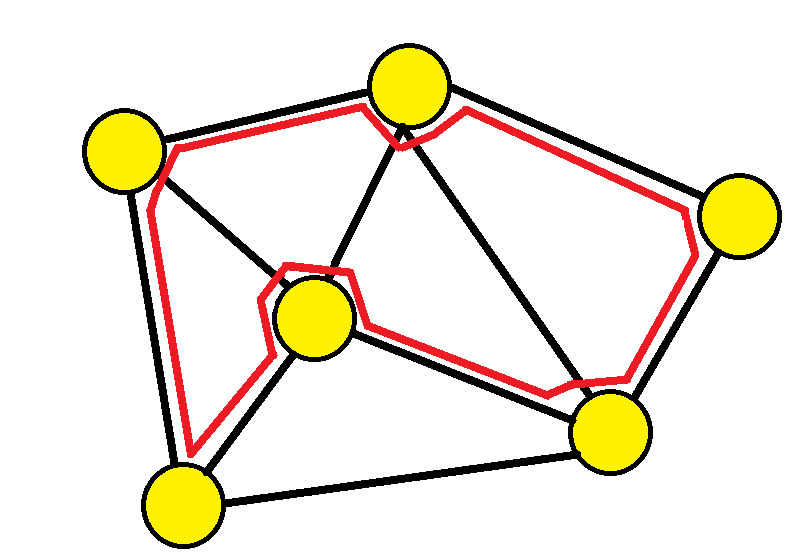
\includegraphics[scale = 0.4]{Hamiltonian.png}
\caption{Hamiltonian Circle.}
\label{fig:figure1label}
\end{figure}

\subsection{Build Hamiltonian Circle}
As we can see, the Hamiltonian Circle can visit every nodes exactly once. As the map in the snake game, the Hamiltonian Circle can visit every single unit exactly once. As Figure \ref{fig:figure2label}, given a initial snake like red arrow including the head direction with the direction of the arrow, we can build a Hamiltonian Circle like yellow path. And then, we can go along the Hamiltonian Circle to eat food successfully until the snake body is full of map. 

\begin{figure}[H]
\centering 
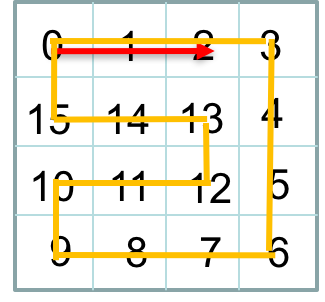
\includegraphics[scale = 0.8]{Picture1.png}
\caption{Hamiltonian Circle in Map.}
\label{fig:figure2label}
\end{figure}

There are two steps to build this yellow Hamiltonian Circle given the initial snake.
\begin{enumerate}
    \item build the shortest path using BFS from head to tail. 
    \item extend the longest path on the foundation of the shortest path above.
\end{enumerate}

First of all, I will build the shortest path using BFS from head to tail. For example, in Figure \ref{fig:figure2label}, putting the node with number 2 into Queue and marking the initial node as distance of 0. Next step, dequeue the node 2 and put the adjacent nodes of number 2 into queue. Marking these adjacent nodes with distance of 1. In the meantime, recording the direction of the parent node. So on and so forth. If I get the tail node in the queue. I can get the path from tail to head by direction of each node's parent nodes. In Figure \ref{fig:figure3label} the third picture is the shortest path using BFS from 2 to 0, head to tail.

Secondly, I will extend the shortest path to a longest path, also known as Hamiltonian Circle in the map. There is a rule in extending the course that if two chosen points are up or down direction, the extending direction will be left or right. For example, in Figure \ref{fig:figure3label}, from picture 3, we can see from head(node2)(1,3), the next points along the shortest path (2,3) has the direction of down from the node2. So I'll extend this two points to the left or right direction. The left direction cannot be extended and the right direction will be chosen. Two points will be extended towards right until to the wall like the path in picture 4. Next, we'll choose next two points (1, 4) and (2,4), but it cannot be extended any direction. Next, we'll choose next two points (2, 4) and (2, 3), the (2, 3) locate in (2, 4) left, so the extending direction is up or down. Down is proper direction. In picture 5 and 6, the result has been shown.

\begin{figure}[H]
\centering 
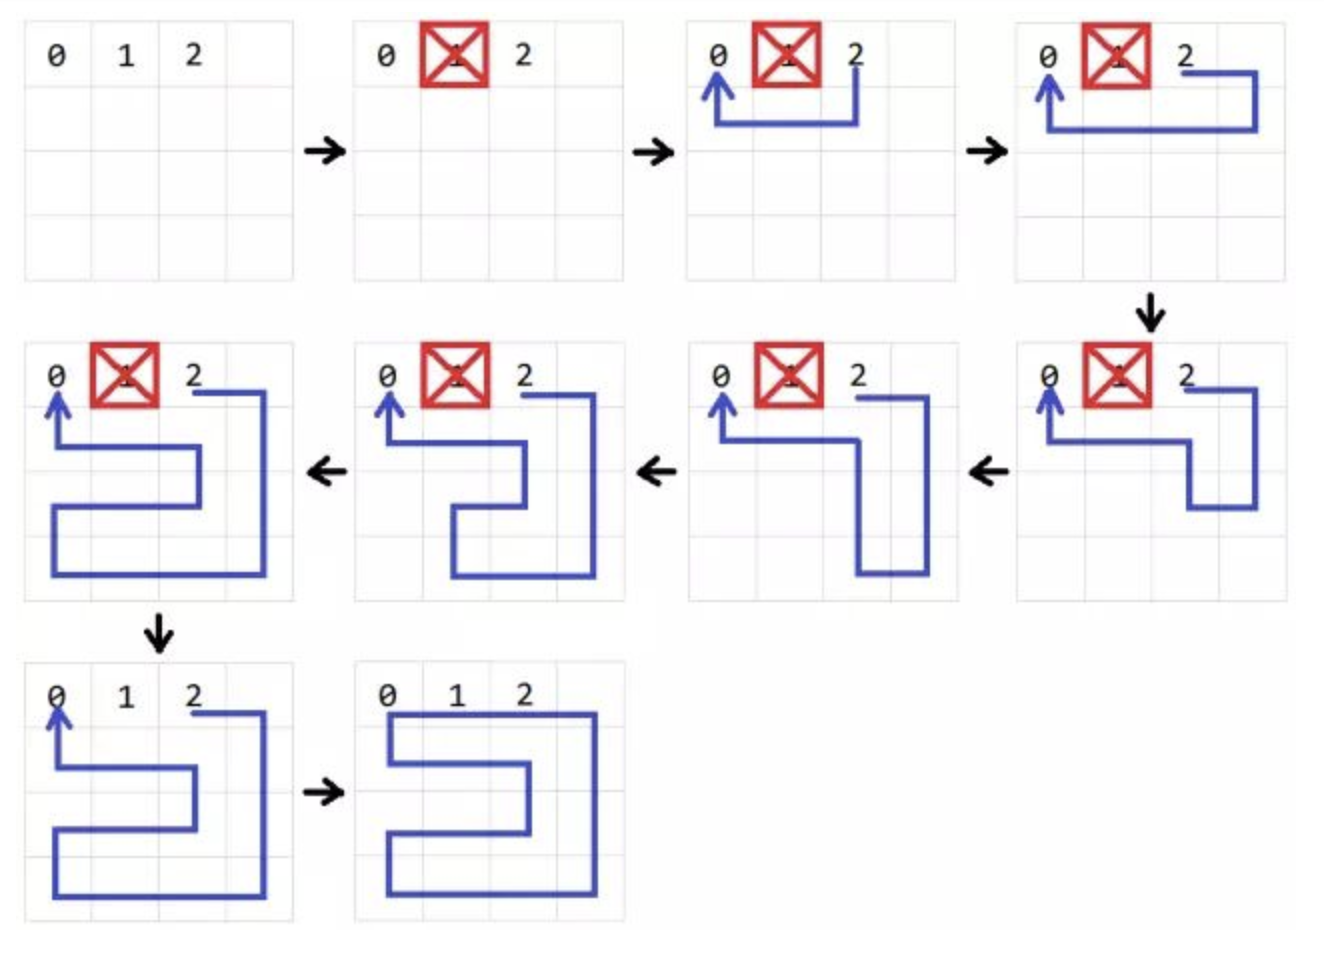
\includegraphics[scale = 0.4]{2.png}
\caption{Build Hamiltonian Circle.}
\label{fig:figure3label}
\end{figure}

Finally, we can get a longest path, which is the Hamiltonian Circle in the map of self-playing snake game.

\section{Shortcuts in Hamiltonian Circle Algorithm}

Although Hamiltonian Circle Algorithm can insure the snake eat every food, it need move much steps in total game. Every time the snake need go along the longest path even the food is near the snake head. In this case, I can choose a shortcut in the early-stage to let the total number of movements become smaller. But it needs more time to judge the next direction. That's a trade-off between movement length and direction judgement time. 

The method we use to choose shortcuts is to find the shortest path between current head position and food using BFS and then judge if this direction available. Using BFS to find shortest path is same as the find shortest path between head and tail in the last section. The main point is the second part, how to judge if we choose this next direction. What we do is to find if the next direction is in the body range between head index and tail index. For example, in Figure \ref{fig:figure4label}, the red arrow is current snake. If the next direction judged by using BFS from head to food(not shown in picture) is down, 1, the number in node is  between the number in the head 14 and the tail 4. In this case, we refuse this direction and use Hamiltonian Circle to go next direction 15. If the next direction is up, 1 is not between 14 and 4, we will accept this direction.  

\begin{figure}[H]
\centering 
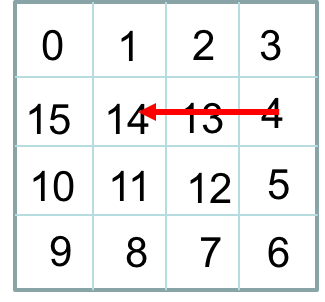
\includegraphics[scale = 0.8]{Picture3.png}
\caption{snake in game.}
\label{fig:figure4label}
\end{figure}

These two algorithm can eat every food until the snake body is full of the map. Two algorithm need build a Hamiltonian Circle when given a initial snake before game starts. Naive Hamilton Algorithm doesn't need extra judgement but need more movements length in entire process. Advanced Algorithm including shortcuts need extra judgements but less movements length. That's a trade-off.

\end{document}